\documentclass[10pt,a4paper]{article}
\usepackage[a4paper,margin=14mm,top=12mm,bottom=14mm]{geometry}
\usepackage{fontspec}
\setmainfont{Liberation Sans}
\usepackage{polyglossia}
\setdefaultlanguage{french}
\usepackage{amsmath}
\usepackage{xcolor}
\usepackage{graphicx}
\usepackage[most]{tcolorbox}
\usepackage{tabularx,booktabs,array,multirow}
\usepackage{enumitem}
\usepackage{fancyhdr}
\usepackage{lastpage}
\usepackage[hidelinks]{hyperref}
\definecolor{uimm}{HTML}{005677}
\definecolor{cyan}{HTML}{13A2DD}
\definecolor{fond}{HTML}{E6F2FA}
\definecolor{ok}{HTML}{2E7D32}
\definecolor{ko}{HTML}{B3261E}
\definecolor{violet}{HTML}{7B1FA2}
\setlength{\parindent}{0pt}
\setlength{\parskip}{3pt}
\setlist{nosep}
\setlist[itemize]{leftmargin=13pt,label=\textcolor{cyan}{\textbullet}}
\newcommand{\titre}[1]{\vspace{5pt}{\color{uimm}\large\bfseries #1}\par\vspace{-3pt}{\color{cyan}\rule{\linewidth}{1.2pt}}\par\vspace{0pt}}
\tcbset{boite/.style={colback=fond,colframe=uimm,boxrule=0.6pt,arc=2pt,left=6pt,right=6pt,top=4pt,bottom=4pt},
        defi/.style={colback=violet!6,colframe=violet,boxrule=0.8pt,arc=2pt,left=6pt,right=6pt,top=4pt,bottom=4pt,
                     title={\bfseries Défi},coltitle=white,colbacktitle=violet,fonttitle=\small}}
\newcommand{\bandeau}[3]{%
\begin{tcolorbox}[colback=uimm,colframe=uimm,arc=2pt,left=4pt,right=8pt,top=4pt,bottom=4pt]
\begin{minipage}[c]{18mm}\setlength{\fboxsep}{1.2pt}\fcolorbox{white}{white}{
\includegraphics[height=16.5mm]{logo_uimm.jpg}}\end{minipage}\hspace{4mm}%
\begin{minipage}[c]{\dimexpr\linewidth-22mm\relax}\color{white}
{\small #1}\\[1pt]{\LARGE\bfseries #2}\\[2pt]{\large #3}\hfill{\small CQPM Technicien qualité}
\end{minipage}
\end{tcolorbox}}
\newcommand{\reponse}[1][1]{\par\vspace{2pt}{\color{gray!60}\foreach \i in {1,...,#1}{\rule{\linewidth}{0.3pt}\par\vspace{9pt}}}}
\usepackage{pgffor}
\pagestyle{fancy}\fancyhf{}
\renewcommand{\headrulewidth}{0pt}
\newcommand{\pied}[1]{\fancyfoot[L]{\footnotesize\color{uimm}#1}\fancyfoot[R]{\footnotesize\color{uimm}Page \thepage{} sur \pageref{LastPage}}}

\usepackage{tikz}
\usepackage{longtable}
\renewcommand{\bandeau}[3]{%
\begin{tcolorbox}[colback=uimm,colframe=uimm,arc=2pt,left=4pt,right=8pt,top=4pt,bottom=4pt]
\begin{minipage}[c]{18mm}\setlength{\fboxsep}{1.2pt}\fcolorbox{white}{white}{
\includegraphics[height=16.5mm]{logo_uimm.jpg}}\end{minipage}\hspace{4mm}%
\begin{minipage}[c]{\dimexpr\linewidth-22mm\relax}\color{white}
{\small #1}\\[1pt]{\LARGE\bfseries #2}\\[2pt]{\large #3}
\end{minipage}
\end{tcolorbox}}
% en-tête d'une fiche : code, titre, question, bloc, durée, organisation, niveau
\newcommand{\entete}[7]{%
\begin{tcolorbox}[colback=uimm,colframe=uimm,arc=2pt,left=4pt,right=6pt,top=4pt,bottom=4pt]
\begin{minipage}[c]{18mm}\setlength{\fboxsep}{1.2pt}\fcolorbox{white}{white}{
\includegraphics[height=16.5mm]{logo_uimm.jpg}}\end{minipage}\hspace{3mm}%
\begin{minipage}[c]{\dimexpr\linewidth-58mm\relax}\color{white}\raggedright
{\small Base SPC · #4}\\[1pt]{\Large\bfseries #1 · #2}\\[2pt]{\itshape #3}
\end{minipage}\hfill
\begin{minipage}[c]{33mm}\color{white}\small\raggedleft
Durée : \textbf{#5}\\ \textbf{#6}\\ Niveau #7 sur 3
\end{minipage}
\end{tcolorbox}}
\newcommand{\tagE}{{\setlength{\fboxsep}{1.5pt}\colorbox{cyan}{\color{white}\scriptsize\bfseries Ellistat}}}
\newcommand{\tagW}{{\setlength{\fboxsep}{1.5pt}\colorbox{uimm}{\color{white}\scriptsize\bfseries Page web}}}
\tcbset{pred/.style={colback=orange!6,colframe=orange!80!black,boxrule=0.6pt,arc=2pt,left=6pt,right=6pt,top=3pt,bottom=1pt,
                    title={\bfseries Je prédis, avant de commencer},coltitle=white,colbacktitle=orange!80!black,fonttitle=\small},
        retenir/.style={colback=fond,colframe=uimm,boxrule=0.6pt,arc=2pt,left=6pt,right=6pt,top=3pt,bottom=3pt,
                    title={\bfseries À retenir},coltitle=white,colbacktitle=uimm,fonttitle=\small},
        plus/.style={colback=violet!6,colframe=violet,boxrule=0.6pt,arc=2pt,left=6pt,right=6pt,top=3pt,bottom=3pt,
                    title={\bfseries Pour aller plus loin},coltitle=white,colbacktitle=violet,fonttitle=\small},
        act/.style={colback=uimm!10,colframe=uimm,boxrule=0.5pt,arc=2pt,left=5pt,right=5pt,top=2pt,bottom=2pt,before skip=7pt,after skip=3pt},
        verif/.style={colback=orange!6,colframe=orange!80!black,boxrule=0.6pt,arc=2pt,left=6pt,right=6pt,top=3pt,bottom=3pt,
                    title={\bfseries À vérifier sur poste avant la première séance},coltitle=white,colbacktitle=orange!80!black,fonttitle=\small}}
\newcommand{\fichier}[1]{\texttt{\small #1}}
\newcommand{\menu}[1]{\textsf{\textbf{#1}}}
\newcommand{\champ}[1]{\rule{#1}{0.3pt}}

\pied{Base SPC · fiche G2 · Un micromètre, plusieurs tolérances}
\begin{document}
\thispagestyle{fancy}
\entete{G2}{Un micromètre, plusieurs tolérances}{Le même micromètre est-il capable pour toutes les tolérances ?}{Mallettes GUNT : plaques et arbres}{60 min}{en groupe}{3}
\begin{tcolorbox}[boite]\textbf{Le but.} Mener une étude R\&R sur dix arbres PT105 (Ø 48 ± 0,2) avec un micromètre 25-50 mm, puis voir comment le \%GRR change quand la tolérance change : l'instrument ne change pas, le jugement si.\par\textbf{Il vous faut.} 10 arbres PT105 numérotés (cote g, Ø 48 ± 0,2) · Un micromètre 25-50 mm · Ellistat et une page web (adresse à l'étape 3)\end{tcolorbox}
\begin{tcolorbox}[pred]Un micromètre, trois ou quatre opérateurs, dix arbres. Le \%GRR par rapport à la tolérance du dessin ($\pm 0{,}2$ mm) sera-t-il sous 10 \% ? Et si la tolérance était $\pm 0{,}05$ mm ?\reponse\end{tcolorbox}
\titre{À faire}
\begin{enumerate}[label=\textcolor{cyan}{\textbf{\arabic*.}},leftmargin=15pt,itemsep=1.5pt]
\item Numéroter les arbres 1 à 10 et tracer un repère au feutre sur le Ø 48 : on mesure toujours au même endroit. Nettoyer les portées du micromètre.
\item Chaque opérateur mesure les 10 arbres dans un ordre mélangé, deux séries, sans regarder ses résultats précédents. Un mesure, un note : 20 valeurs par opérateur, soit 60 en tout avec trois opérateurs et 80 avec quatre.
\item \tagW\ Ouvrir la page « L'opérateur compte-t-il ? » à l'adresse suivante :\par \href{https://sjaubert.github.io/000_OI/SPC/Pages/L_operateur_compte-t-il.html}{\nolinkurl{https://sjaubert.github.io/000_OI/SPC/Pages/L_operateur_compte-t-il.html}}\par $T = 0{,}40$ (47,8 à 48,2) ; résolution de votre micromètre. Choisir d'abord le nombre d'opérateurs (3 ou 4) : un changement efface la grille. Saisir les 20 valeurs de chaque opérateur (60 en tout à trois, 80 à quatre), Calculer. Relever \%GRR, EV, AV et le nombre de catégories distinctes.
\item \tagW\ Dans la même page, changer seulement $T$ : 0,20 puis 0,10 puis 0,05. Calculer à chaque fois et noter le \%GRR. Ne pas toucher aux mesures.
\item \tagE\ \menu{Gage R\&R}, onglet \menu{Mesures}, bouton « ajouter un gage R\&R ». Remplir : Nom ; Produits 10 ; Opérateurs 3 ou 4 ; Répétitions 2 (Ellistat propose 3) ; Type de tolérance Bilatéral, Tolérance min 47,8 et max 48,2 ; Méthode de calcul \textbf{ANAVAR} ; K 3. Valider, puis « Voir Plus » : vérifier que les deux tolérances sont bien là.
\item \tagE\ Onglet \menu{Mesure} : saisir les mesures de chaque opérateur. Onglet \menu{Analyse} : lire GRR\%, Cpc et le nombre de catégories distinctes. Comparer à la page.
\item À la main : tolérance minimale pour laquelle le micromètre serait capable (\%GRR au plus 10 \%) : $T_{\min} = 60 \times \text{GRR}$.
\end{enumerate}
\vspace{3pt}{\renewcommand{\arraystretch}{1.5}\begin{tabularx}{\linewidth}{|l|*{3}{>{\centering\arraybackslash}X|}}\hline
\textbf{Tolérance T (mm)} & \textbf{\%GRR (page)} & \textbf{Cpc = 100 / \%GRR} & \textbf{Verdict}\\\hline
0,40 (± 0,2) &  &  & \\\hline
0,20 (± 0,1) &  &  & \\\hline
0,10 (± 0,05) &  &  & \\\hline
0,05 (± 0,025) &  &  & \\\hline
\end{tabularx}}\par
\newpage
\titre{J'observe, je décide}
\begin{enumerate}[label=\textcolor{cyan}{\textbf{Q\arabic*.}},leftmargin=22pt]
\item Que devient le \%GRR quand $T$ est divisé par 2 ? Pourquoi ?\reponse[2]
\item Répétabilité (EV) ou reproductibilité (AV) : laquelle pèse le plus ? Que contrôler en premier ?\reponse[2]
\item $T_{\min} = \champ{16mm}$ mm. Le dessin impose $T = 0{,}4$ mm : le micromètre est-il capable pour la cote g ? Et pour une cote de $\pm 0{,}05$ mm ?\reponse[2]
\item Les arbres ont-ils changé entre les quatre lignes du tableau ? Les opérateurs ? Qu'est-ce qui a changé ?\reponse[1]
\end{enumerate}
\begin{tcolorbox}[retenir]La capabilité d'un instrument se juge par rapport à une tolérance. EV et AV restent les mêmes : le \%GRR est inversement proportionnel à $T$.\end{tcolorbox}
\begin{tcolorbox}[plus]Les dix arbres de ce lot sont-ils très différents entre eux ? Cherchez dans le tableau Résultats d'Ellistat la part de la variation due aux pièces, et comparez-la à la part due à la mesure.\end{tcolorbox}
\providecommand{\carre}{\fbox{\rule{0pt}{1.1ex}\rule{1.1ex}{0pt}}}
\begin{tcolorbox}[boite,left=5pt,right=5pt,top=3pt,bottom=3pt]\footnotesize
\textbf{\color{uimm}Lire le plan GUNT (dernière page).} Le cartouche du plan est écrit en allemand et en anglais. À la ligne « Allgemeintoleranzen / General tolerance », on lit \textbf{ISO 2768-mK}. Cela veut dire : toute cote \textbf{sans écart écrit} a la tolérance générale de la classe \textbf{m} (« medium »), donnée par le tableau ci-dessous. Une cote \textbf{avec un écart écrit} garde cet écart, et la tolérance générale ne s'applique pas. Limite haute = nominal + écart supérieur. Limite basse = nominal + écart inférieur. \O\ : diamètre. \carre{} : carré, on lit son côté. « A-A », « B-B » : coupes. Les symboles d'état de surface et d'arêtes, en bas à droite, ne servent pas dans cette fiche.
\par\vspace{6pt}\noindent\renewcommand{\arraystretch}{1.2}\setlength{\tabcolsep}{4pt}
\begin{tabular}{|l|c|c|c|c|c|}\hline
\textbf{Dimension nominale (mm)} & 0,5 à 3 & au-delà de 3 à 6 & au-delà de 6 à 30 & au-delà de 30 à 120 & au-delà de 120 à 400\\\hline
\textbf{Écart de la classe m (mm)} & $\pm 0{,}1$ & $\pm 0{,}1$ & $\pm 0{,}2$ & $\pm 0{,}3$ & $\pm 0{,}5$\\\hline
\end{tabular}
\par\vspace{1pt}{\scriptsize Source : ISO 2768-1:1989, tolérances générales des dimensions linéaires, reprises dans la fiche GUNT « PT105f Tolérances ».}
\par\vspace{4pt}\textbf{Les cotes de cette fiche}\par\vspace{2pt}
\begin{tabularx}{\linewidth}{|c|>{\raggedright\arraybackslash}X|>{\raggedright\arraybackslash}X|}\hline
\textbf{Cote} & \textbf{Ce que le plan écrit} & \textbf{Écart à utiliser}\\\hline
$g$ & \O\ 48 avec $\pm 0{,}2$ & écrit sur le plan : $\pm 0{,}2$ \\\hline
\end{tabularx}
\end{tcolorbox}
\vfill{\footnotesize\color{uimm}\textbf{Ressources de la base :}\par L'opérateur compte-t-il ? (page) : \href{https://sjaubert.github.io/000_OI/SPC/Pages/L_operateur_compte-t-il.html}{\nolinkurl{https://sjaubert.github.io/000_OI/SPC/Pages/L_operateur_compte-t-il.html}}\par Données de secours (3 opérateurs) : \href{https://sjaubert.github.io/000_OI/SPC/Pages/Donnees_a_copier.html\#rrarbres}{\nolinkurl{https://sjaubert.github.io/000_OI/SPC/Pages/Donnees_a_copier.html}}\par Données de secours (4 opérateurs) : \href{https://sjaubert.github.io/000_OI/SPC/Pages/Donnees_a_copier.html\#rrarbres4}{\nolinkurl{https://sjaubert.github.io/000_OI/SPC/Pages/Donnees_a_copier.html}}}
\newpage
\titre{Plan de l'arbre PT105}
{\small Pour lire ce plan et ses tolérances, voir l'encadré « Lire le plan GUNT » de la page précédente.\par}\vspace{2pt}
\begin{center}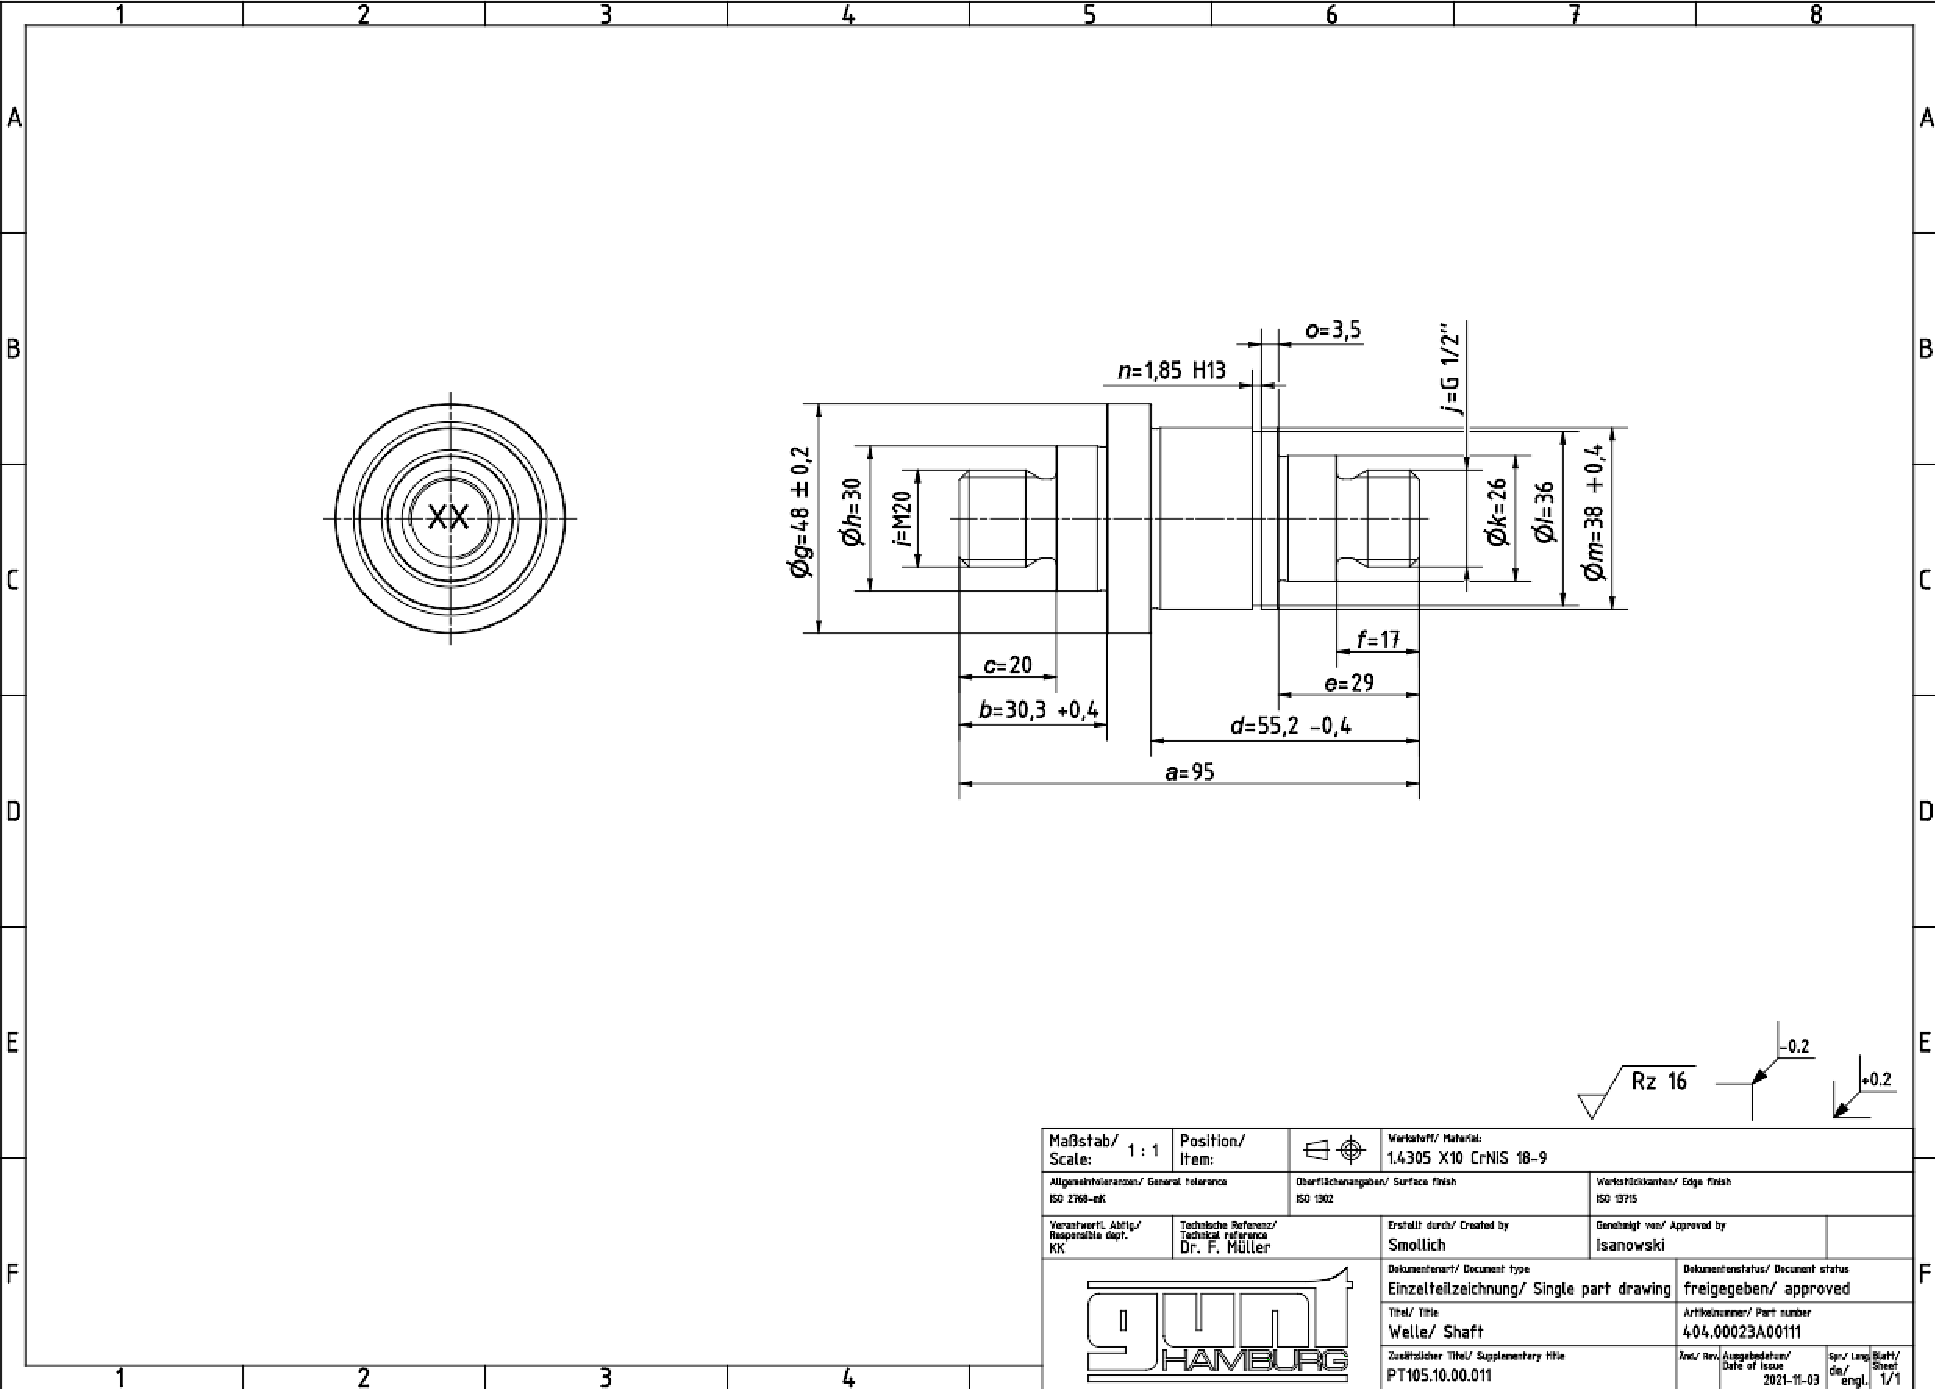
\includegraphics[width=0.90\textheight,height=0.97\linewidth,keepaspectratio,angle=90]{plan_arbre_PT105.pdf}\end{center}
\vfill{\footnotesize\color{uimm}Plan : GUNT Hamburg, Welle (arbre), dessin PT105.10.00.011.}
\end{document}